\chapter{Regularization, Model Selection and Model Evaluation}
\section{Regularization}\label{chap:regularization}

Throughout the course we have discusses multiple hypothesis classes and learners for choosing an hypothesis $h_s\in\Hc$ from a given hypothesis class $\Hc$. In most of these cases choosing $h_S$ was based on minimizing some cost function $\Fc_S\left(h\right)$ over $h\in\Hc$. This means that $h_S\coloneqq\Ac_0\left(S\right)$ is given by: $$ h_S\coloneqq\underset{h\in\Hc}{argmin} \Fc_S\left(h\right) $$

The function $\Fc$ measures how well $h$ fits the training sample $S$. We can call $\Fc_S\left(h\right)$ the \textbf{fidelity term}. We have seen a few examples for such learners already:
\begin{itemize}
	\item In linear regression, $\Fc_S\left(h\right)$ measures the \textbf{RSS}.
	\item In logistic regression, $-\Fc_S\left(h\right)$ is the \textbf{likelihood} of the model (which we want to maximize).
	\item In SVM, $-\Fc_S\left(h\right)$ is the \textbf{margin} of the hyperplane (which we want to maximize).
\end{itemize}
~\\
With the simplest example for learners that minimize a cost function are of course the \textbf{ERM} learners. In any ERM based learner, we define some loss function $\ell\left(\cdot,\cdot\right)$ and define the empirical risk induced by $\ell$, with respect to the training sample $\trainset$ to be: $$ L_S\left(h\right)=\frac{1}{m}\sum^m_{i=1}\ell\left(h\left(\x_i\right),y_i\right) $$
For all of these the fidelity term $\Fc_S\left(h\right)$ is the empirical risl $L_S\left(h\right)$. ~\\

For the different hypothesis classes we have also discussed how their richness and expressiveness governs the bias-variance tradeoff. If the hypothesis class $\Hc$ is ``too large``, we are concerned that minimizing $\Fc$ over $\Hc$ may lead to over-fitting. Namely, we are concerned our learner will output an hypothesis $h_S$ which will not generalize well, as it is too well adapted to the particular training sample $S$.~\\

One way to solve this problem would be to restrict $\Hc$. However, in such a case we are deliberately harming our performance. Instead, we would like to keep $\Hc$ large, but find a way to tell our learner $\Ac_0$ ``Prefer simpler hypotheses but if you find a complex one that is \textit{really} worth it - take it``. To achieve this, we change the optimization problem that $\Ac_0$ uses to choose $h_S$. We introduce an additional term to the problem. We choose $\lambda\geq 0$ and define the learner $\Ac_\lambda:S\mapsto\Hc$ by: $$ h_S\coloneqq \underset{h\in\Hc}{argmin}\, \Fc_S\left(h\right)+\lambda\Rc\left(h\right) $$
The term $\Rc$ is called the \textbf{regularization term}. If choosing $\Rc$ wisely then $\Rc\left(h\right)$ will measure the ``complexity`` of the hypothesis $h$. The more complicated the hypothesis $h$, the larger $\Rc\left(h\right)$ will be.


So we see that in minimizing $ \Fc_S\left(h\right)+ \lambda \Rc\left(h\right)$ we now have a \textbf{trade-off}:
\begin{itemize}
	\item On one hand, more complicated $h$, the better it can describe the training sample $S$, so the fidelity term $\Fc_S\left(h\right)$ will be smaller.
	\item On the other hand, the more complicated $h$, the larger $\Rc\left(h\right)$ will	be. 
\end{itemize}
~\\
And conversely, the simpler $h$, the larger the fidelity term $\Fc_S\left(h\right)$ (as it won't be able to describe the training sample very well) but the smaller
$\Rc\left(h\right)$ will be. So $\lambda$ is a parameter the coverns the trade-off:

\begin{itemize}
	\item For $\lambda=0$, we have no regularization and are back to finding a minimizer of $\Fc_S\left(h\right)$.
	\item For $\lambda \to\infty$, the minimization problem pays no attention to the fidelity term and just wants to find the simplest possible $h\in\Hc$.
	\item Any finite value $\lambda\in(0,\infty)$ defines a specific trade-off between the need for fidelity (small $\Fc_S\left(h\right)$) and the need for simplicity
	of $h$ (small $\Rc\left(h\right)$).
\end{itemize}
~\\
So, when we add regularization to the learner $\Ac_0:S\mapsto\text{argmin}_{h\in\Hc} \Fc_S\left(h\right)$, we won't find a minimizer of $\Fc_S\left(h\right)$ over $\Hc$. We are hoping that a minimizer of the regularized objective function $\Fc_S\left(h\right)+ \lambda \Rc\left(h\right) $ (which does not minimize $\Fc_S\left(h\right)$) will generalize better. This is because, the larger the value of $\lambda$, the simpler this minimizer will be.
\\~\\
We therefore get a \textbf{family} of learners $\{\Ac_\lambda\}_{\lambda\in[0,\infty)}$. The regularization parameter $\lambda$ controls the bias-variance tradeoff: for
$\lambda=0$ we get the most variance and least bias (most complicated $h$); for $\lambda\to\infty$ we get the least variance and most bias (simplest $h$).

\begin{remark}
We already saw one example for regularization - Soft SVM. Recall that the Soft-SVM classifier classifies using the half-space $\w^\perp$ where $\w$ is a solution to the optimization problem:
\begin{eqnarray*}
	& \text{minimize}   &  \lambda \norm{\w}^2 + \frac{1}{m}\sum_i \xi_i \\
	& \text{subject to} & y_i \cdot \left( \inprod{\x_i}{\w} +b \right) \geq 1-\xi_i  \,\,\text{and}\,\, \xi_i\geq 0 
\end{eqnarray*}
Here, the fidelity term is $\norm{\w}^2$. The smaller $\norm{\w}^2$, the better we fit the training data (in the sense of larger margin). As the total margin is proportional to $1/\norm{\w}$, so that minimizing  $\norm{\w}^2$ means maximizing the margin. The regularization term is  $\frac{1}{m}\sum_i \xi_i$. The smaller this term is, the ``simpler`` the hypothesis since we allow less violations of the margin.
~\\
Note that here $\lambda$ is placed on the fidelity term and not on the regularization term.
\end{remark}

\todo{ Regression Trees - Add definitions to Decision Trees under classification. Add adaptation of algorithm as exercise }
\todo { Add pruning of trees - Maybe add it under classification. Just refer to here for ideas (and teach when getting here)}

\subsection{Subset Selection}
Let us revisit linear regression and the OLS estimator. We defined the hypothesis class of linear regression \ref{eqn:lin_reg_h}: $$ \Hreg\coloneqq\left\{h: h\left(x_1,\ldots,x_d\right)=w_0+\sum^d_{i=1}x_iw_i,\,\, w_0,w_1,\ldots,w_d\in\R\right\} $$ and given a regression problem $\X, \y$, we select $h_S\in\Hreg$ by using the OLS estimator (which we have derived both as ERM for the square loss and using Maximum Likelihood assuming Gaussian noise). When doing so we assumed that the training sample size $m$ aws not smaller than the number of features $d$, and even preferred that $m\gg d$, since of $m\sim d$ the variance of the OLS estimator can be large.
\\~\\
However, in modern learning problems based on $d$ features, very often we are in a situation where $d$ can be quite large. Linear regression was invented when features were measured and recorded manually. In the last few decades it became very easy to collect features and record them automatically, and a typical regression problem can easily have $d\sim m$ or even $d\gg m$. 
\\~\\
When $d\sim m$ or, worse, $d\gg m$, we will have correlated features. The coefficients fitted by linear regression will be poorly determined. For example, a large positive coefficient for some feature can be canceled out by a large negative coefficient for an almost-parallel feature. So the linear regression learner we saw should not be used for $m\sim d$ and cannot be used for $d>m$.
\\~\\
Therefore, we would like to devise a method where we keep only a subset of the features. Let $k\leq d$ be the desired number of features, then we could solve the following optimization problem:

\begin{equation}
\begin{array}{cl}
\text{minimize}   &  \norm{\y-\X\w}^2 \\
\text{subject to} &  \sum_{i=1}^d \indc{\w_i \neq 0} = k
\end{array}
\label{eqn:best_subset}
\end{equation}
That is, find a coefficients vector $\w$ that minimizes the $RSS$ under the restriction of using exactly $k$ features. This is exactly what the Best-Subset Selection algorithm does (\todo{reference to pseudo}). It iterates all possible combinations of $k$ features, fits an OLS model for each, and returns the model (i.e. a vector $\w$) achieving the lowers loss. A related, but not equivalent, problem introduces a regularization term over the number of used features:

\begin{equation}
\underset{w_0\in\R, \w\in\R^d}{argmin} \norm{w_0\vv{1} + \X\w - \y}^2 + \lambda\norm{\w}_0
\label{eqn:l0_reg}
\end{equation}
where $\norm{\w}_0\coloneqq \sum_i \indc{\w_i \neq 0}$. Notice how in both optimization problems we do not include the intercept ($w_0$) in the restriction on the number of features as the intercept is not one of the features per se.
\\~\\\todo{Add pseudo of Best-subset-selection}

As $k$, the number of features in the model, gives some measure of the complexity of the hypothesis, we can think of the family of learners $\left\{\Ac^{best-subset}_k | 0\leq k\leq d\right\}$. As we change $k$ we move on the bias-variance trade-off. Unfortunately, even for a single value of $k$, we must go over all ${d \choose k}$ subsets of $k$ features. This is an NP-Hard problem and as such cannot be solved efficiently. 

\todo{ Add Forward/Backaward Selection algorithms? }


\subsection{Ridge ($\ell_2$) Regularization}
In addition to the computational challenges imposed by the best-subset regularization, it also often suffers from high variance as features are included or excluded based on the single specific training-set we have. To cope with both problems, we often use different \textit{shrinkage methods} where we restrict the values of the coefficients, shrinking them towards zero. One such method is the Ridge regression, which imposes a $\norm{\cdot}_2$ penalty on the coefficients:

\begin{equation}
\ridge\coloneqq\underset{w_0\in\R, \w\in\R^d}{argmin} \norm{w_0\vv{1} + \X\w - \y}^2 + \lambda\norm{\w}_2^2\quad \lambda\geq 0
\label{eqn:l2_reg}
\end{equation}

So $\lambda\geq 0$ is the complexity parameter that controls the amount of shrinkage. For $\lambda=0$ we get the OLS solution (the standard linear regression solution). As $\lambda \rightarrow \infty$ we penalize more and more on the size of the coefficients vector, driving the solution $\ridge\rightarrow 0$. As $\lambda$ increases the bias increases (we restrict ourselves to specific sets of solutions) and variance decreases (solution is not based solely on training-set).

\begin{figure}[!h]
	\centering
	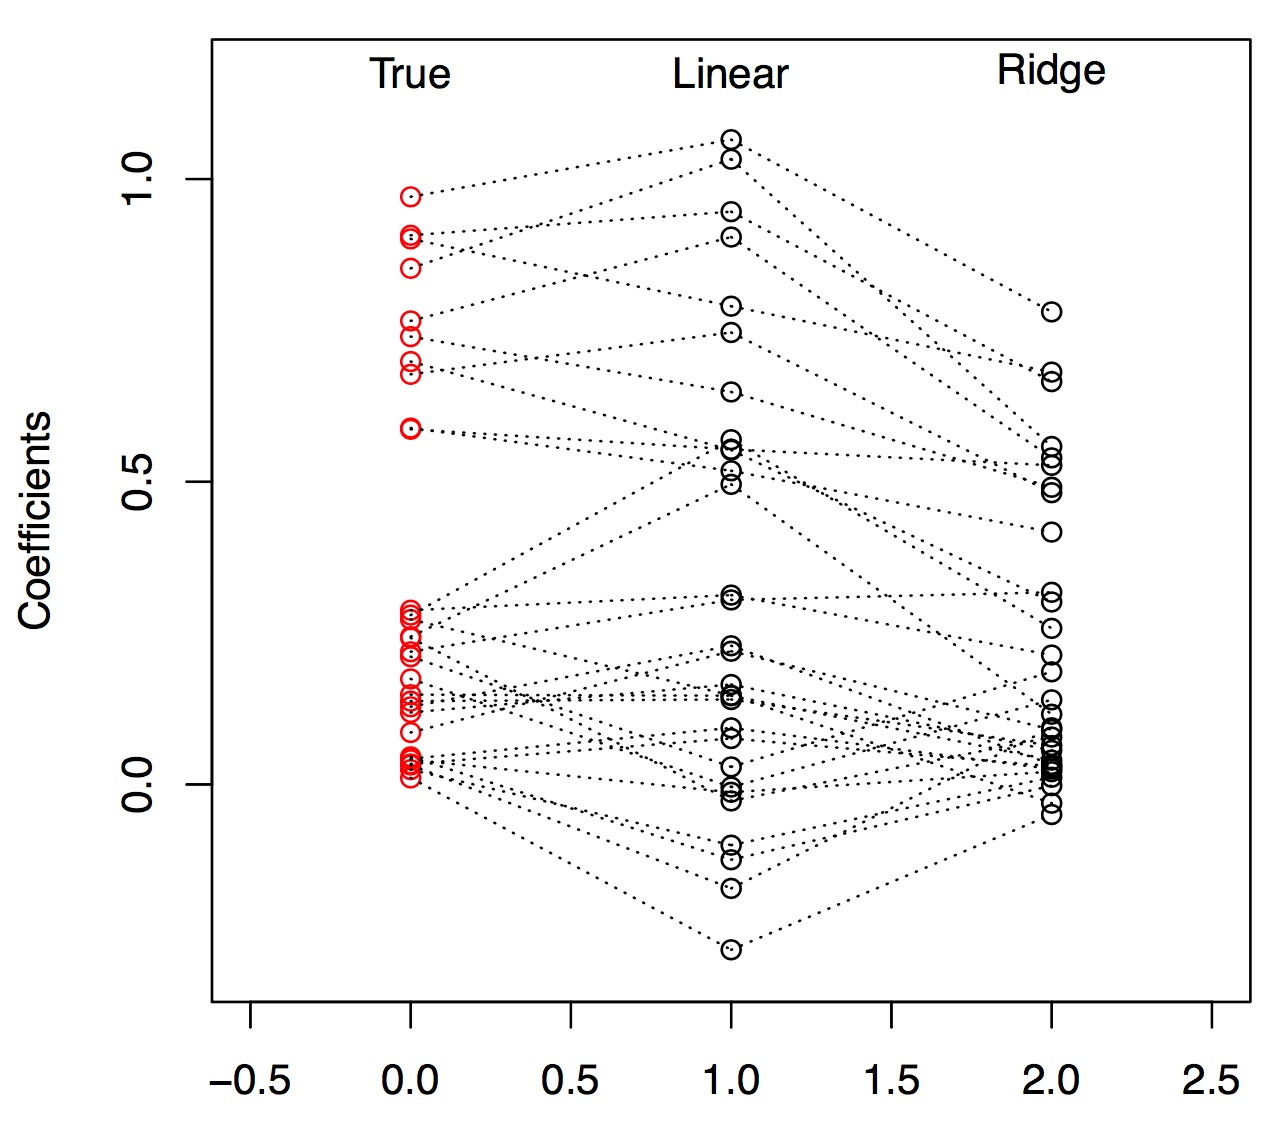
\includegraphics[width=0.5\textwidth]{chapters/regularization.model.selection/figures/ridge_coefs.jpeg}
	\caption{\todo{Add caption}}
\end{figure}

\todo{better removal of penalty over intercept - ESL - page 64}
Though the Ridge optimization problem is a convex problem, and specifically a case of quadratic programming, it has in-fact a neat closed form.

\begin{theorem}
Let $\X,\y$ be a regression problem and let $\lambda\geq 0$. The solution for the Ridge Regression problem \ref{eqn:l2_reg} is given by: $$ \ridge\coloneqq \left(\X^\top \X + \lambda I_d\right)^{-1}\X^\top\y $$
\end{theorem}
\begin{proof}
For $\lambda=0$ then indeed $\ridge=\ols$. Let $\lambda>0$ then to find a minimizer of the objective function, we begin with equating it's derivative in each coordinate to zero: 
$$ \frac{\partial \norm{w_0\vv{1} + \X\w - \y}^2 + \lambda\norm{\w}_2^2}{\partial \w_k}= -2\sum^m_{i=1} \left(y_i-\sum^d_{j=1}\x_{ij}\w_j\right)\x_k + 2\lambda \w_k = 0\quad i=1,\ldots,d $$
which in matrix notation is:
$$
\begin{array}{c}
\left[\X^{\top}\y\right]_{k}-\left[\X^{\top}\X\w\right]_{k}-\left[\lambda\w\right]_{k}=0\\
\Downarrow\\
\X^{\top}\y=\X^{\top}\X\w+\lambda I_{d}\w\\
\Downarrow\\
\X^{\top}\y=\left(\X^{\top}\X+\lambda I\right)\w
\end{array}
$$
\end{proof}
As $\X^\top \X+\lambda I$ is non-singular (even if $\X^\top \X$ is not of full rank) it has an inverse and hence the solution is given by: $$\ridge=\left(\X^{\top}\X+\lambda I\right)^{-1}\X^\top\y $$

Ridge regression could also be solved using the SVD method for OLS weights, which can be generalized. 

\begin{claim}
Let $\X,\y$ be a regression problem and $\X=U\Sigma V^\top$ be the SVD of $\X$. The Ridge estimator is given by: $$ \ridge=U\Sigma_\lambda V^\top\y, \quad \left[\Sigma_\lambda\right]_{ii}=\frac{\sigma_i}{\sigma_i^2+\lambda} $$
\end{claim}
\begin{proof}
Let us replace $\X$ with its SVD:
$$
\begin{array}{cclcl}
\ridge & = & \left(\X^{\top}\X+\lambda I\right)^{-1}\X^{\top}\y & = & \left(\left(U\Sigma V^{\top}\right)^{\top}U\Sigma V^{\top}+\lambda I\right)^{-1}\left(U\Sigma V^{\top}\right)^{\top}\y\\
& = & \left(V\Sigma U^{\top}U\Sigma V^{\top}+\lambda I\right)^{-1}V\Sigma U^{\top}\y & = & \left(V\Sigma^{2}V^{\top}+\lambda VV^{\top}\right)^{-1}V\Sigma U^{\top}\y\\
& = & V\left(\Sigma^{2}+\lambda I\right)^{-1}V^{\top}V\Sigma U^{\top}\y & = & V\Sigma_{\lambda}U^{\top}\y
\end{array}
$$
where we denote $\left[\Sigma_\lambda\right]_{ii}=\frac{\sigma_i}{\sigma_i^2 + \lambda}$ and $\sigma_i$ are the singular values of $\X$.
\end{proof}

\todo{Explain that is a biased estimator but reduces the variance. Maybe take question from homework and put here instead. Might be beneficial to show this in recitation instead } 
\begin{figure}[!h]
	\centering
	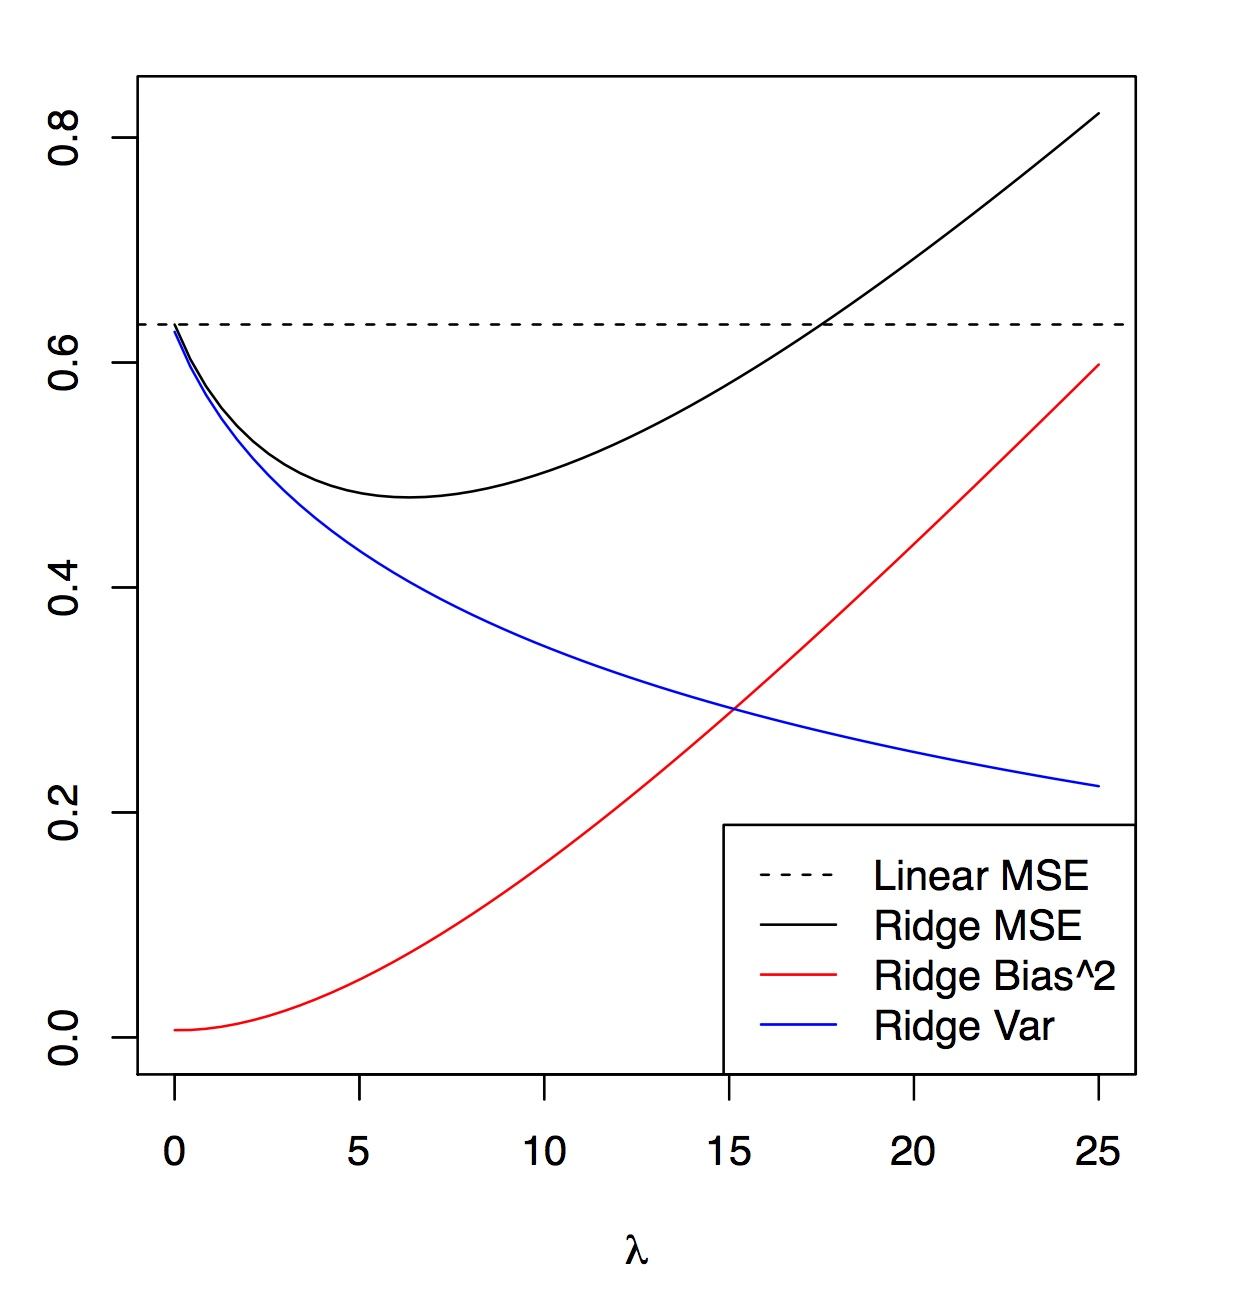
\includegraphics[width=0.5\textwidth]{chapters/regularization.model.selection/figures/ridge_bias_variance.jpeg}
	\caption{\todo{Add caption}}
\end{figure}

\todo{Add regularization path explanation}


\subsection{Lasso ($\ell_1$) Regularization}
By introducing the ridge regularizer we were able to apply linear regression when $d>m$ or when $\X^\top\X$. In addition, we saw that even though the ridge estimator is a biased estimator it achieves a lower variance compared to the OLS estimator. However, as evident from the regularization path, the ridge estimator does not do what best-subset does. That is, it cannot \textbf{select} a specific subset of features to use for regression.
\\~\\
The \textit{Least Absolute Shrinkage and Selection Operaotr} (Lasso) attempts to achieve exactly that. This regularization method uses the $\ell_1$ norm rather than the $\ell_2$ norm:
\begin{equation}
\lasso\coloneqq\underset{w_0\in\R, \w\in\R^d}{argmin} \norm{w_0\vv{1} + \X\w - \y}^2 + \lambda\norm{\w}_1\quad \lambda\geq 0
\label{eqn:l1_reg}
\end{equation}
This optimization problem is still convex and therefore can be solved efficiently. Similar to Ridge setting $\lambda=0$ we get the OLS solution and setting $\lambda\rightarrow\infty$ will shrink the coefficients $\lasso\rightarrow 0$. However the manner of shrinkage is very different between the two problems. The lasso solution, \lasso, is \textbf{sparse}. That is, it has zero entries in the vector. Therefore, the larger $\lambda$, typically the more zeros \lasso will have, effectively defining a subset of features that are used by the model (a feature corresponding a coefficient of zero is not used by the model). We often refer to this subset of features as the "active set". As we are considering problems where $d$ can be very large, it is hard to interpret the model. Thus, the Lasso has an important advantage in interpretability over Ridge, as it selects for us a subset of variables.

\begin{figure}[!h]
	\centering
	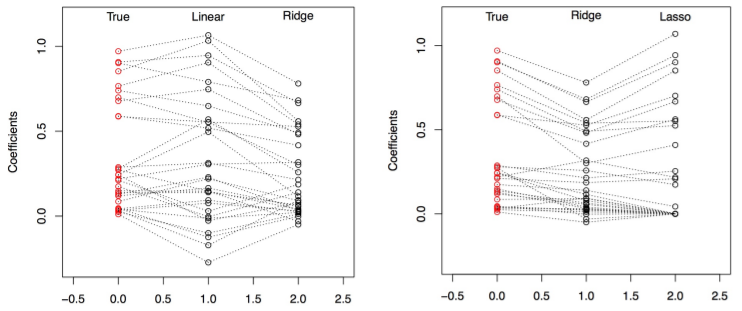
\includegraphics[width=0.5\textwidth]{chapters/regularization.model.selection/figures/coef_ridge_lasso.png}
	\caption{\todo{Add caption}}
\end{figure}

\todo{Add comparison of regularization path between ridge and lasso}


\subsubsection{Convexity vs. Sparsity}
We have discussed three regularization methods for regression problems using the terms: $\norm{\cdot}_0,\norm{\cdot}_1,\norm{\cdot}_2$ (which we will also denote by $\ell_0,\ell_1,\ell_2$). We saw that for both $\ell_1,\ell_2$ we still have a convex optimization problem whereas for the $\ell_0$ term the problem is non-convex. In addition, we stated that unlike $\ell_2$, when using $\ell_1$ we typically introduce sparsity to the solution. Let us expand this discussion for the $L_q$ familty of norms:
\begin{equation}
\text{For } 0<q\in\R,\,x\in\R^d\quad \norm{x}_q\coloneqq \left(\sum_{i=1}^d \left(x_i\right)^q\right)^{\frac{1}{q}}
\label{eqn:lq_norm}
\end{equation}
If applying any norm in this family as the regression regularization term then:
\begin{itemize}
	\item Sparsity - For any $q\leq 1$ we typically obtain sparse solutions and therefore our active set of features is smaller than $d$.
	\item Convexity - For any $q\geq 1$ the optimization problem (when we use the RSS loss as the fidelity term) is convex. Therefore the problem can be solved efficiently.
\end{itemize}

The \textit{Lasso} regression uses $q=1$ and as such achieves \textbf{both} sparsity and convexity. But why are $L_{q\leq 1}$ norms obtain their sparsity? This is in fact based on the shapes of their unit balls.
\begin{definition}
For a norm $\norm{\cdot}$ on $\R^d$, a ball of radius $\rho$ (around the origin) is the set: $B_{\rho}\coloneqq\left\{\w\in\R^d|\norm{\w}\leq\rho\right\}$. The unit ball of a norm is the ball of radious $\rho=1$.
\end{definition}

For $L_{q>1}$, such as in the case of the Euclidean norm, the unit ball has no corners. In contrast, the unit balls of $L_{q\leq 1}$ have corners. Specifically, the unit ball of the $\ell_1$ norm over $\R^d$ has $2d$ corners.

\begin{figure}[!h]
	\centering
	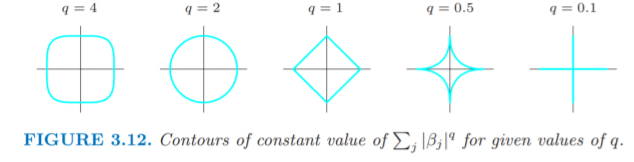
\includegraphics[width=0.5\textwidth]{chapters/regularization.model.selection/figures/unit_balls.png}
	\caption{\todo{Add caption}}
\end{figure}

Now, let us revisit the Ridge and Lasso optimization problems. Instead of the unconstrained forms seen in \ref{eqn:l1_reg} and \ref{eqn:l2_reg} consider the equivalent constraint versions:
$$
\begin{array}{ll|lll}
\text{minimize }w_0\in\R,\w\in\R^d & \norm{w_0\vv{1}+\X\w-y}^2 & \quad & \text{minimize }\w_0\in\R,\w\in\R^d & \norm{w_0\vv{1}+\X\w-y}^2 \\
\text{subject to} & \norm{\w}_2^2\leq \rho & &\text{subject to} & \norm{\w}_1\leq \rho\\
\end{array}
$$

Now, let us fix some $\rho\in\R$ and ask where will we find the $\widehat{\w}_\rho^{ridge}$ and $\widehat{\w}_t^{lasso}$ solutions. As the fidelity term is a quadratic form in $\w$, its level sets are ellipsoids. Suppose $\rho$ is very large, so there is effectively no constrain, the solution of the minimization problem will be the OLS solution. As we restrict the solution more and more, by making $\rho$ smaller and smaller, we are limiting the solution to be inside the norm ball. By definition, the solution will be found where one of the level sets of the fidelity term intersects with the ball of radius $\rho$. When we consider the $L_{q\leq 1}$ norms (such as the $\ell_1$ in Lasso) this intersection typically happens at one of the corners of the norm ball. As these corners take place on the axes they correspond to \textbf{sparse} solutions.

\begin{figure}[!h]
	\centering
	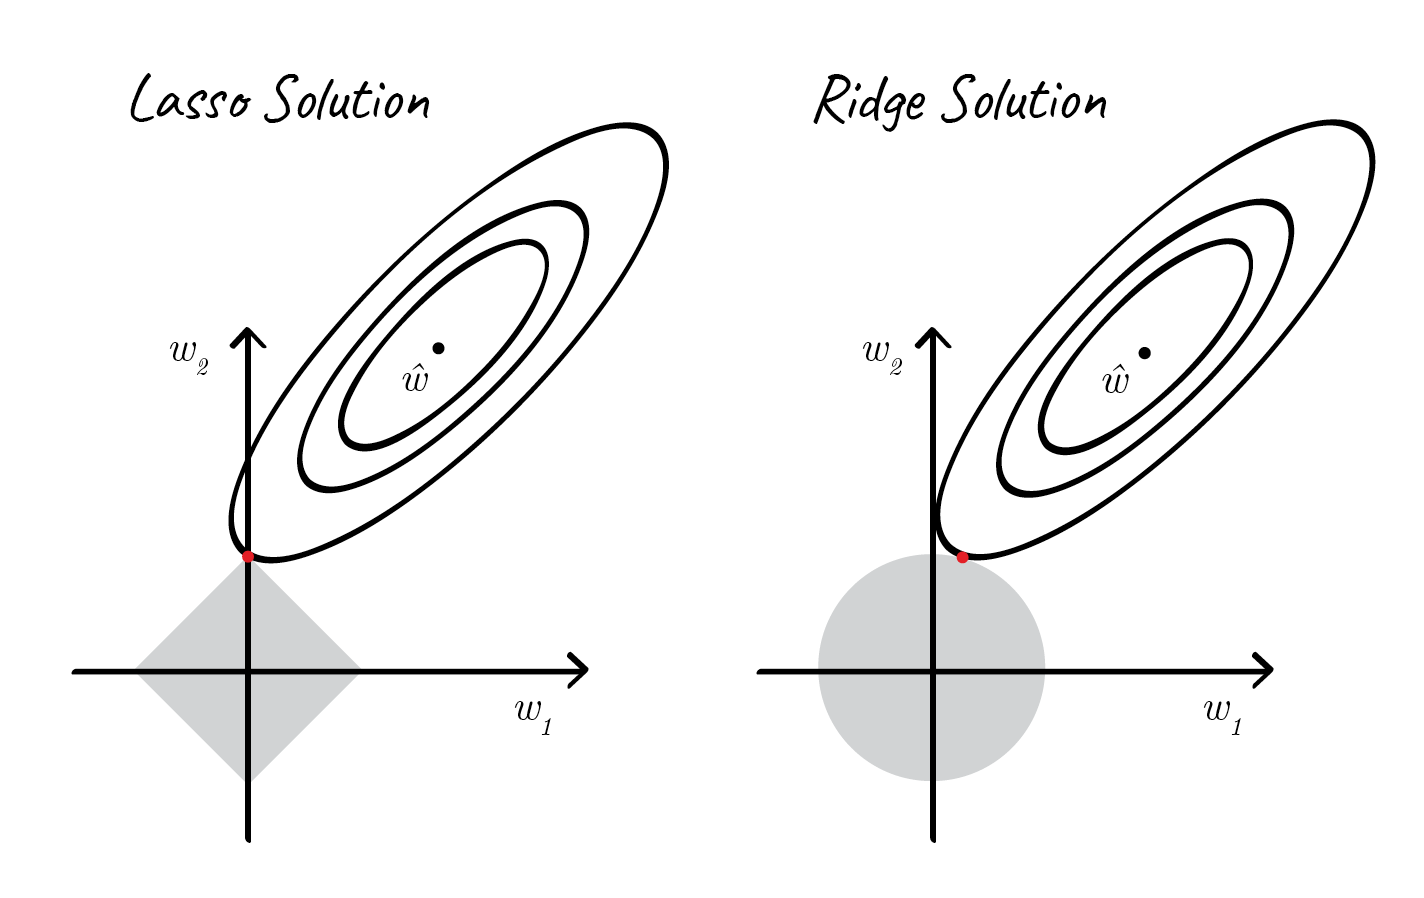
\includegraphics[width=0.5\textwidth]{chapters/regularization.model.selection/figures/6.1.png}
	\caption{\todo{Add caption}}
\end{figure}


\subsection{The Orthogonal Design Case}
Here is another way to understand why Lasso solutions are sparse. Consider the case where all features are orthogonal to each other, namely $\X^\top\X=I_d$. In some sense, this is the simplest setup for regression problems, where we can write $\y$ as a linear combination of \textbf{orthonormal} vectors. This is also known as an orthogonal design. In such setup, we have a closed form solution for $\bestsubset,\ridge,\lasso$ based on the $\ols$ solution.
\\~\\
Let us define two \textit{thresholding} functions.
\begin{definition}
Let the hard- and soft-threshold (at $\lambda$) be the functions $\eta_\lambda^{hard},\eta_\lambda^{soft}:\R\rightarrow\R$ defined by:$$
\begin{array}{cc|cc}
\eta^{hard}_\lambda\coloneqq\indc{\left|x\right|-\lambda}\cdot x & \quad & \quad &
\begin{array}{ccc}
\eta_\lambda^{soft}\coloneqq sign\left(x\right)\left[\left|x\right|-\lambda\right]_+=
\begin{cases}
	x-\lambda & x\geq \lambda	\\
	0 & \left|x\right|<\lambda\\
	x+\lambda & x\leq \lambda\\
\end{cases}
\end{array}
\end{array}
$$
\end{definition}
These functions define a manner of shrinking an input value $x$ towards $0$, depending on $\lambda$. The hard-thresholding zeros inputs in the range of $\left(-\lambda,+\lambda\right)$ and leaves inputs outside of this range unchanged. The shoft-thresholding shrinks inputs out of the $\left(-\lambda,+\lambda\right)$ range, and zeros inputs that are within the range.

\begin{claim}
	Let $X,y$ be an orthogonal design matrix and a response vector. Denote $\widehat{w}$ the OLS solution. The lasso regularization optimization problem takes the form of $\widehat{w}^{lasso}\left(\lambda\right) = \eta_{\lambda}^{soft}\left(\widehat{w}\right)$ 
\end{claim}
\begin{proof}
	Recall that the OLS solution is $\hat{\w} = (\X^\top\X)^{-1}\X\y = \X\y$. 
	Write the objective function:
	$$
	\begin{array}{ccl}
	f_{\ell_{1}}\left(\w\right)=\frac{1}{2}\left|\left|\y-\X\w\right|\right|_{2}^{2}+\lambda\left|\left|\w\right|\right|_{1} & = & \frac{1}{2}\left( \left|\left|\y\right|\right|^2 - 2\y^\top \X\w + \w^\top \X^\top\X\w \right) + \lambda\left|\left|\w\right|\right|_{1} \\
	& = & \frac{1}{2}\left(\left|\left|\y\right|\right|^2 + \left(\w^{\top}-2\widehat{\w}^{\top}\right)\w \right) + \lambda\left|\left|\w\right|\right|_{1} \\
	& = & \frac{1}{2}\left|\left|\y\right|\right|^{2}+\sum_{j=1}^{d}\left(\frac{1}{2}\w_{j}^{2}-\widehat{\w}_{j}\w_{j}+\lambda\left|\w_{j}\right|\right)\\
	& = & \frac{1}{2}\left|\left|\y\right|\right|^{2}+\sum_{j=1}^{d}\left(\frac{1}{2}\w_{j}-\widehat{\w}_{j}+\lambda sign\left(\w_{j}\right)\right)\w_{j}
	\end{array}
	$$
	Let us minimize the expression for each $\w_{j}$ taking into account the value of $\lambda$. So: 
	$$
	\begin{array}{c}
	\frac{\partial\frac{1}{2}\left|\left|\y-\X\w\right|\right|+\lambda\left|\left|\w\right|\right|_{1}}{\partial \w_{j}}=\frac{\partial\left(\frac{1}{2}\w_{j}-\widehat{\w}_{j}+\lambda sign\left(\w_{j}\right)\right)\w_{j}}{\partial \w_{j}}=\w_{j}-\widehat{\w}_{j}+\lambda sign\left(\w_{j}\right)=0\\
	\Downarrow\\
	\w_{j}=\widehat{\w}_{j}-\lambda sign\left(\w_{j}\right)
	\end{array}
	$$
	
	
	Let us divide into cases:
	\begin{itemize}
		\item If $\left|\widehat{\w}_{j}\right|<\lambda$ then $\w_{j}=0$. That it because:
		\begin{itemize}
			\item If $\w_{j}<0$ then $0>\w_{j}=\widehat{\w}_{j}+\lambda$, which $\forall\left|\widehat{\w}_{j}\right|<\lambda$ the right-hand side is positive in contradiction.
			\item If $\w_{j}>0$ then $0<\w_{j}=\widehat{\w}_{j}-\lambda$, which $\forall\left|\widehat{\w}_{j}\right|<\lambda$ the right-hand side is negative in contradiction.
		\end{itemize}
		\item If $\widehat{\w}_{j}\geq\lambda$ then $\w_{j}=\widehat{\w}_{j}-\lambda sign\left(\w_{j}\right)$ which is valid only for $\w_{j}\geq0$ which means that $\w_{j}=\widehat{\w}_{j}-\lambda$.
		\item If $\widehat{\w}_{j}\leq-\lambda$ then $\w_{j}=\widehat{\w}_{j}-\lambda sign\left(\w_{j}\right)$ which is valid only for $\w_{j}\leq0$ which means that $\w_{j}=\widehat{\w}_{j}+\lambda$.
	\end{itemize}
	Putting it all together we got that:
	$$
	\w_{j}\left(\widehat{\w}_{j},\lambda\right)=\begin{cases}
	\widehat{\w} - \lambda & \widehat{\w}\geq\lambda\\
	0 & \left|\widehat{\w}\right|<\lambda\\
	\widehat{\w}+\lambda & \widehat{\w}\leq\lambda
	\end{cases}
	\quad\Longrightarrow\quad\widehat{\w}_{j}^{lasso}\left(\lambda\right)=\eta^{soft}_\lambda\left(\widehat{\w}_{j}^{ols}\right)
	$$
\end{proof}

Similarly, we can obtain the Best-Subset and Ridge solutions:
$$
\begin{array}{ccc}
\bestsubset & \coloneqq & \eta_{\sqrt{\lambda}}^{hard}\left(\ols\right)\\
\ridge & \coloneqq & \ols / \left(1+\lambda\right)
\end{array} $$
Namely, in the orthogonal design setup we can obtain the different solutions by applying a \textbf{univariate shrinkage function} to each coordinate of $\ols$ separately. Observe that in this case:
\begin{itemize}
	\item The Best-Subset sets some coefficients to zero and leaves the rest untouched.
	\item The Lasso solution sets some coefficients to zero and shrinks the rest by $\lambda$.
	\item The Ridge solution simply multiplies by a scalar.
\end{itemize}
Therefore, for the Best-Subset and Lasso solutions, the solutions' sparsity grows  as $\lambda$ grows.

\begin{figure}[!h]
	\centering
	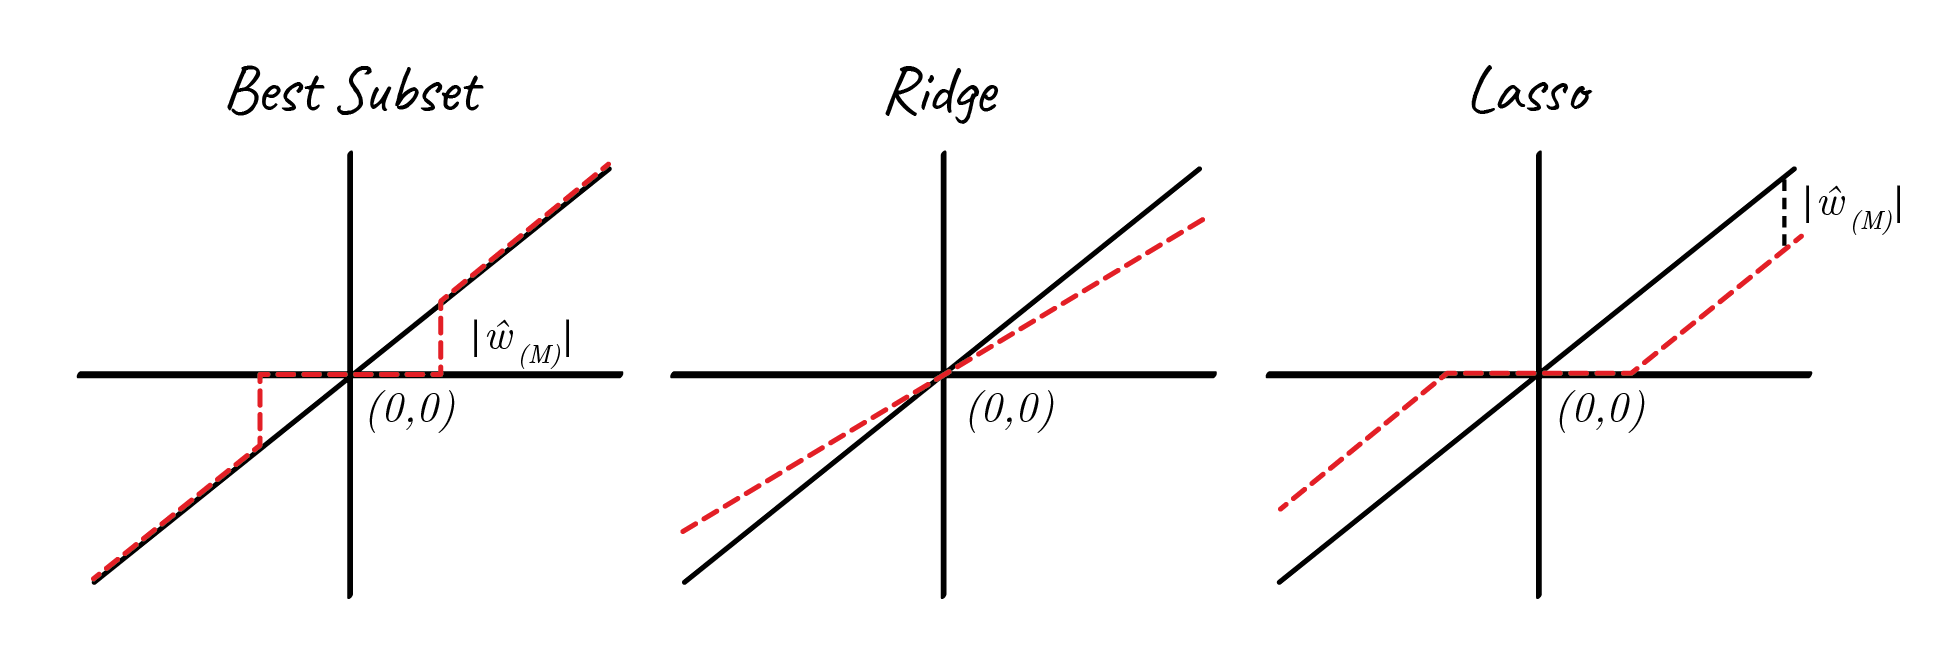
\includegraphics[width=1\textwidth]{chapters/regularization.model.selection/figures/6.2.png}
	\caption{\todo{Add caption}}
\end{figure}

\subsection{Regularized Logistic Regression}
We have seen a few different (linear) regression methods using regularization. We can also apply these regularization terms to other regression models such as the logistic regression. Similarly to linear regression, if $m\sim d$ or $d>m$, also for logistic regression optimization will be numerically unstable, might have parallel feature vectors with large coefficients of opposite signs and hard for interpretation. All these problems are alleviated by adding a regularization term.
\\~\\
Recall that the logistic regression classifier find the coefficients vector by solving:
$$ \widehat{\w} \coloneqq \underset{w_0\in\R,\w\in\R^d}{argmax}\sum^m_{i=1}\left[y_i\left(\inprod{\x_i}{\w}+w_0\right)-log\left(1+e^{w_0+\inprod{\w}{\x_i}}\right)\right]$$
We can add the $\ell_1$ regularization term to the above fidelity term to obtain the $\ell_1$-regularized logistic regression classifier:
$$ \widehat{\w} \coloneqq \underset{w_0\in\R,\w\in\R^d}{argmax}\sum^m_{i=1}\left[y_i\left(\inprod{\x_i}{\w}+w_0\right)-log\left(1+e^{w_0+\inprod{\w}{\x_i}}\right) + \lambda \norm{\w}_1\right]$$
This is still a convex optimizatoin problem, and fast specialized solvers are available. The $\ell_1$-regularized logistic regression classifier is a very powerful classifier over $\Xc=\R^d$. It has low variance, we are able to control the bias-variance tradeoff (by choosing $\lambda$) and is it very interpretable.

\section{Model Selection and -Evaluation}
So far, we have discussed several learning algorithms and meta-algorithms that can be applied over the existing learning algorithms. In the coming section we will be answering the following questions:\\
\begin{itemize}
	\item \underline{How to \textbf{select} a model}? For different algorithms we have described the existance of a family of learners where we defined some ``tuning`` hyper-parameter. For example, $k$ the number of neighbors used in the $k$-NN algorithm; the maximal tree depth and pruning regularization in CART; or the regularization lambda in soft-SVM and the different regularized linear- and logistic- regression problems.
	\\~\\
	In the case of meta-algorithms such as bagging or boosting, in addition to the base learners' tuning parameters, we need to choose the number of bagging/bootstrapping iterations $B$. If we are using de-correlation in bagging, there might be additional tuning parameters (e.g the number $k$ of allowed coordinated for a split in the Random Forest algorithm).\\~\\
	\item \underline{How to \textbf{estimate} the performance of a chosen model}? Before applying the chosen model on new samples we would like to estimate how will it perform on a new independent set of samples. If our estimation of the generalization error for the selected model is poor, perhaps we are working with the wrong learning algorithm for our problem, and should therefore select a different candidate. In addition, often we are interested in known how our chosen learner will perform before we begin using it.
\end{itemize}
~\\The performance we would like to estimate, which would also influence the selection of the model, is the generalization error. Assume some loss function $\ell\left(\cdot,\cdot\right)$ then we defined the empirical risk of an hypothesis $h:\Xc\rightarrow\Yc$ simple as the average loss over the training sample: $$ L_S\left(h\right)\coloneqq\frac{1}{m}\sum^m_{i=1}\ell\left(h\left(\x_i\right),y_i\right)\quad \trainset$$
The generalization error (also reffered to as \textit{test error}), that is the predicted error over an independent sample set depends on our data-generation model:
\begin{itemize}
	\item \underline{No data-generation model}: If we are not assuming any model to describe how the data is generated we simply define the generalization error as the average loss over the test set: $$ L\left(h\right)\coloneqq \sum^{\left|T\right|}_{i=1} \ell\left(h\left(\x_i\right),y_i\right)$$
	\item\underline{Probability distribution over $\Xc$ and unknown labeling function $f:\Xc\rightarrow\Yc$}: When assuming a model as the PAC model, the generalization error is the expected error over sampling from the distribution: $$ \E_{x\sim\Dc}\left[\ell\left(h\left(\x\right),f\left(\x\right)\right)\right] $$
	\item\underline{Probability distribution over $\Xc\times\Yc$}: When assuming a model as the Agnostic PAC model, the generalization error is the expected error over sampling a sample-label pair from the distribution: $$ L_\Dc\left(h\right) \coloneqq \E_{\left(\x,y\right)\sim\Dc}\left[\ell\left(h\left(\x\right),y\right)\right]$$
\end{itemize}

\todo{Better conned Bias-Variance part - or not include it as we already covered it in the Bias-Variance chapter?}

Once we understand what is the generalization error, the next step is to find a way to \textbf{correctly estimate} it. Suppose we follow the following procedure: Given a supervised batch learning setting, where our training sample is $\trainset$, let us perform model selection and -evaluation over a family of learning algorithms $\left\{\Ac_\alpha\right\}$ simply by using $S$:
\begin{itemize}
	\item \underline{Training}: Train each model over $S$ to obtain $\left\{h_\alpha\coloneqq \Ac_\alpha\left(S\right)\right\}$
	\item\underline{Model selection}: Choose the best model by using $\alpha^*\coloneqq argmin_\alpha L_S\left(h_\alpha\right)$
	\item\underline{Model evaluation}: Estimate the generalization error of the chosen trained model $h_{\alpha^*}$ as $L_\Dc\left(h_{\alpha^*}\right)=L_S\left(h_{\alpha^*}\right)$. Namely, the generalization error estimator is just the model's empirical risk over $S$.
\end{itemize}
~\\This procedure will yield poor results. The selection is based on the empirical error of the model. As we have already seen in the bias-variance trade-off, the generalization error can be represented as the sum of both the bias- and the variance of the model. The model we select $\alpha^*$ will adapt as much as possible (under the restriction to some $\Hc$) to the training data. The more variance the learner has, the more it will be able to adapt to the particular properties of $S$. Out generalization error estimator will suffer from \textbf{optimism} (which is in fact the technical term for the difference between the empirical risk and generalization error). Thus, we need to devise a different method to estimate the generalization error. One that will suffer less from optimism.

\subsection{Train-Validation-Test Scheme}
The naive approach of using the finite training set $S$ both for training the model and estimating it's future performance yields poor results. Suppose we had infinitely many samples, could we have done better? In such scenario we could use three different sets $S$ (training), $V$ (validation) and $T$ (testing):
\begin{itemize}
	\item\underline{Training}: Train each model over $S$ to obtain $\left\{h_\alpha\coloneqq \Ac_\alpha\left(S\right)\right\}$
	\item\underline{Model selection}: Choose the model minimizing the loss over the validation set: $\alpha^*\coloneqq argmin_\alpha L_V\left(h_\alpha\right)$
	\item\underline{Model evaluation}: Estimate the generalization error of the chosen trained model $h_{\alpha^*}$ as the loss over the test set. That is, $L_\Dc\left(h_{\alpha^*}\right)\coloneqq L_T\left(h_{\alpha^*}\right)$.
\end{itemize}

The introduction of a third set of samples, the validation set, which is used to select the final model decouples the training- from the model selection- stages. This provides us with an unbiased estimator of the generalization error which we can also use to bound the generalization error.

\begin{claim}
Let $h_S\coloneqq\Ac\left(S\right)$ be the hypothesis returned by a learner over the training sample $S$, and let $V$ be a new (``fresh``) iid samples from $\Dc$. The empirical risk of $h_S$ over $V$ is an unbiased estimator of the generalization error of $h_S$.
\end{claim}
\begin{proof}
Denote $m_V=\left|V\right|$. As the sample are identically distributed then:
$$
\begin{array}{ccl}
\underset{{V\sim\Dc^{m_V}}}{\E} \left[L_V\left(h_S\right)\right] & = & \frac{1}{m_V}\overset{m_V}{\underset{i=1}{\sum}} \E_{V\sim\Dc^{m_V}}\left[\ell\left(h_S,\left(\x_i,y_i\right)\right)\right]  \\
& = & \frac{1}{m_V}\overset{m_V}{\underset{i=1}{\sum}} \E_{\left(\x_i,y_i\right)\sim\Dc}\left[\ell\left(h_S,\left(\x_i,y_i\right)\right)\right] \\
& = & L_\Dc\left(h_S\right)
\end{array}
$$
\end{proof}
For the following, let us assume that the loss function is \textit{bounded}. If the loss function is unbounded, the generalization error cannot be bounded. Suppose the loss function is bounded by 1.
\begin{corollary}
The generalization error of $h_S$ is bound by: $$ \Prob\left[\left|L_V\left(h_S\right)-L_\Dc\left(h_S\right)\right|\leq \sqrt{\frac{\log\left(2/\delta\right)}{2m_V}}\right] \geq 1-\delta $$
\end{corollary}
\begin{proof}
Recall from Hoeffding's inequality that if $X_1,\ldots,X_m$ are a set of bounded iid random variables such that $0\leq X_i\leq 1$ and $\overline{X}=\frac{1}{m}\sum X_i$, then: $\Prob\left[\left|\overline{X}-\E\left[\overline{X}\right]\right|\geq \eps\right]\leq 2\exp\left(-2m\eps^2\right)$. As $V$ is a set of iid samples denote $$Z_i\coloneqq \left(\x_i,y_i\right)$$ the random variable of the selected pair. Since the samples are iid then $Z_1,\ldots,Z_{m_V}$ are iid too. Next, denote $$ X_i\coloneqq \ell\left(h_S,Z_i\right) $$ the random variable of the loss over the $Z_i$ sample. It holds that $ X_1,\ldots,X_{m_V} $ are a set of iid random variables such that $0\leq X_i \leq 1,\quad i=1,\ldots,m_V$. Notice, that for $\overline{X}=\frac{1}{m_V}\sum X_i=L_V\left(h_S\right)$, as $L_V\left(h_S\right)$ is an unbiased estimator of the generalization error, we directly get that:
$$ \Prob\left[\left|L_V\left(h_S\right)-L_\Dc\left(h_S\right)\right|\geq \eps \right] \leq 2\exp\left(2m_V\eps^2\right) $$
By setting $\eps=\sqrt{\frac{1}{2m_V}\ln\frac{2}{\delta}}$ we conclude that:
$$ \Prob\left[\left|L_V\left(h_S\right)-L_\Dc\left(h_S\right)\right|\leq \sqrt{\frac{\log\left(2/\delta\right)}{2m_V}}\right] \geq 1-\delta $$
\end{proof}

\subsection{Cross Validation}
In reality, splitting our finite set of samples into three sets is problematic. In the great majority of cases we are unwilling to decrease the size of our training set. We have already seen that training over a smaller set yields inferior results. Therefore, designating an additional portion of our limited number of samples just for validation isn't feasible. Instead we would like to come up with some method to use $S$ for training but still do proper model selection and -evaluation.
\\~\\
Potentially the simplest method to do so is cross-validation (CV). Instead of thinking about $S$ as a single set, let us think of it as a disjoint union of $K$ equality sized sets, named folds. Then, for each $k=1,\ldots,K$, we fit a model using all samples of $S$ \textbf{except} samples belonging to the $k$'th fold. We then use the $k$'th fold to calculate the prediction error of the fitted model. Finally we report the estimated generalization error across all $K$ folds. This method is called $k$-fold Cross Validation. The $k$'th fold, which is not used for training but only for evaluating the trained model functions as an unbiased estimator for the generalization error.
\\~\\
So this method can be used for selecting the  tuning parameters. For each candidate $\Ac_\alpha$, we train it $k$ times according to the CV procedure, each time leaving out one of the $k$ folds. Then we choose $\alpha$ (and as such the learner $\Ac_\alpha$) whose average error (over the $k$ validation sets) was lowest.
\begin{figure}[!h]
	\centering
	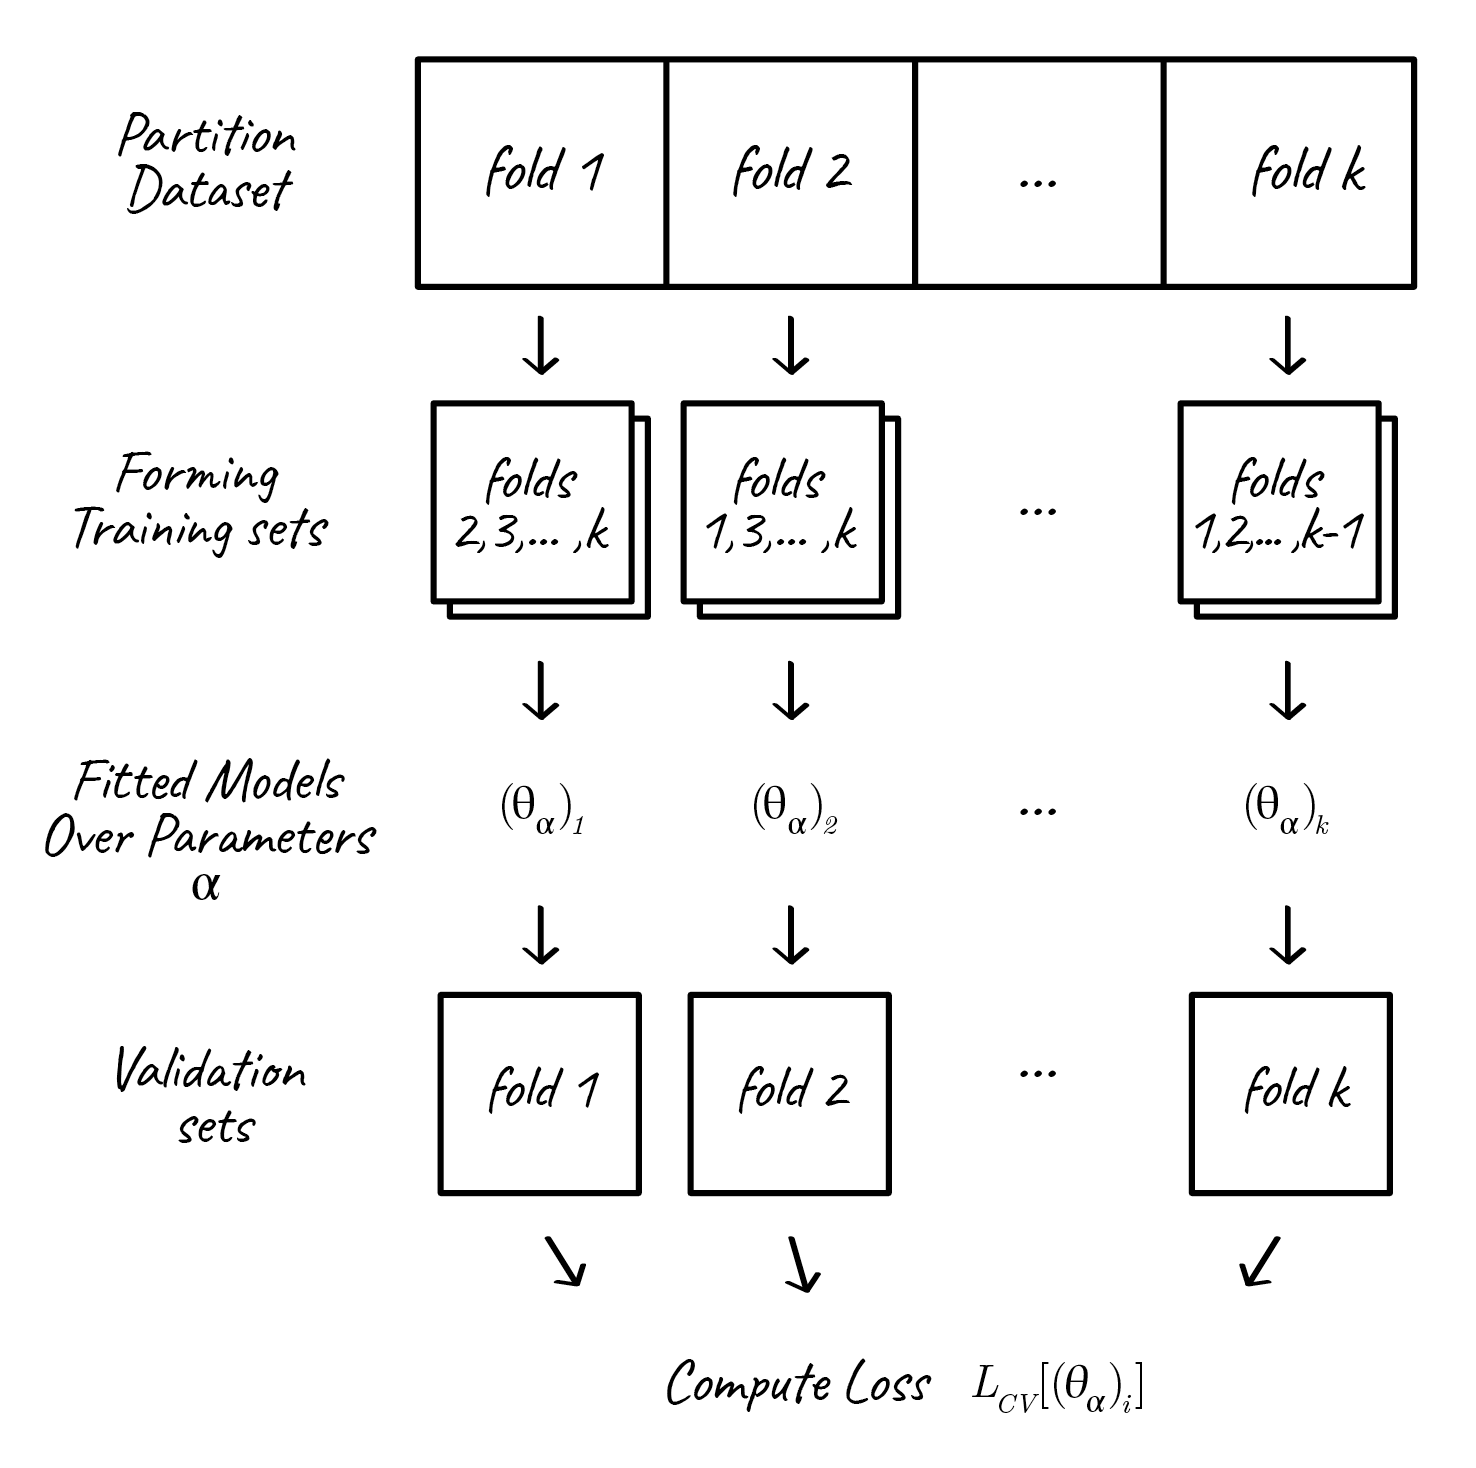
\includegraphics[width=0.7\textwidth]{chapters/regularization.model.selection/figures/6.3.png}
	\caption{\todo{Add caption}}
\end{figure}
Once we finished the model selection phase using CV, and have a fully specified learner $\Ac$, we train $\Ac$ \textbf{again} on the entire training sample $S$. This way we are still able to train $\Ac$ on as many points as possible.
\\~\\
The last step is using CV for model evaluation. Once we have a final, fully specified learner $\Ac$, we run $k$-fold CV and report the average error and standard deviation over the $k$ folds. In this manner we supply both an estimation of the generalization error and a measure of accuracy for this estimate.
\begin{figure}[!h]
	\centering
	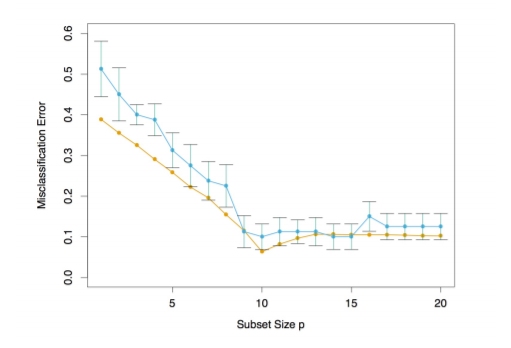
\includegraphics[width=0.5\textwidth]{chapters/regularization.model.selection/figures/cv_estimator.png}
	\caption{\todo{Add caption}}
\end{figure}
\\~\\
\paragraph{Choosing $k$, the number of folds} By using CV we have now introduced another "hyper-hyper"-parameter. How should we choose the value for $k$? If $k=1$ then there is no CV. If $k=2$ we split the data into two equally sized folds where we train only one half of the data. Therefore, the reported CV error will be larger than the true generalization error (also known out-of-sample error). If $k=m$, the sample size, it is called \textbf{leave-one-out} CV. Generally, if $k$ is small we may be training on a dataset too small. As such the CV error may be biased upwards. On the other hand, if $k$ is large, the training samples are very similar to each other. As such the trained models are highly correlated, which might introduce high variances.

\begin{remark}
Another consideration when using CV is computational. Since we train each model $k$ times, the larger $k$, the more computations we perform.
\end{remark}

\subsection{Bootstrap}
In \autoref{bootstrap} we introduced the idea of bootstrapping, where by using re-sampling with replacement we can seemingly create new datasets. This method can also be used for estimating the generalization error using just the single training sample $S$. To do so let $\Ac_\alpha$ be some learner and $B\in\N$ the number of bootstrap samples to create. Very similar to the CV approach we could now:
\begin{itemize}
	\item Draw a bootstrap sample $S^{\left(b\right)}$ by sampling $m$ samples from $S$ with replacement.
	\item By sampling $S^{\left(b\right)}$ we also obtain an independent test set $T^{\left(b\right)}\coloneqq S\setminus S^{\left(b\right)}$ being the samples not chosen in the $b$-th bootstrap sample. These samples are also called the \textbf{out-of-bag} samples.
	\item Train $\Ac$ over $S^{\left(b\right)}$ to aquire an hypothesis $h_S$ and test it over $T^{\left(b\right)}$.
	\item Finally, report the estimated mean and standard deviation of the generalization error, as measured over the $B$ test sets.
\end{itemize} 
\subsection{Common Model Selection Mistakes}
There are two very common mistakes when performing model evaluation using either of the methods seen before. The first causes over-estimation of the generalization error while the other causes under-estimation of the generalization error.
\subsubsection{Over-estimating Generalization Error}
Consider a family of learners $\left\{\Ac_\alpha\right\}$ over which cross-validation was used in order to determine $\alpha$ and obtain the fully specified learner $\Ac$. When each family member was trained it was done using a training set smaller than $S$. For $k$ the number of folds used and $m$ the number of samples in $S$, each model was trained using $m\left(k-1\right)/k$ samples.
\\~\\
Now, recall that successful learning depends on the number of training samples. When discussing PAC theory we defined the sample complexity as the minimal number of samples required to learn an hypothesis from a given hypothesis class, given some $\eps,\delta$. If $m$ samples is a sufficient training size, but $m\left(k-1\right)k$ is not, we cannot guarantee the bounds over the generalization error. In such cases we will estimate the generalization error \textbf{too high}, namely over-estimate it.
\\~\\
To better determine the number of folds, we would like to have an hypothetical learning curve (\autoref{learning_curve}) for the model in question. Such a curve will capture the essence of the sample complexity function. Given a certain number of training samples the curve shows the expected success rate. Using think curve over a training set $S$ with $m$ samples, we can calculate the effective training set size when using $k$-fold cross-validation for a certain $k$. If the effective training size remains in the saturated area of the graph the estimated generalization error using cross-validation would not differ by much from the real generalization error. However, if the effective training size is where the slope of the graph is steep, we do not have a sufficient amount of training samples and will suffer from over-estimating the generalization error.

\todo{But how to estimate the graph? Maybe add a lab? or maybe add it here?}

\begin{figure}[!h]
	\centering
	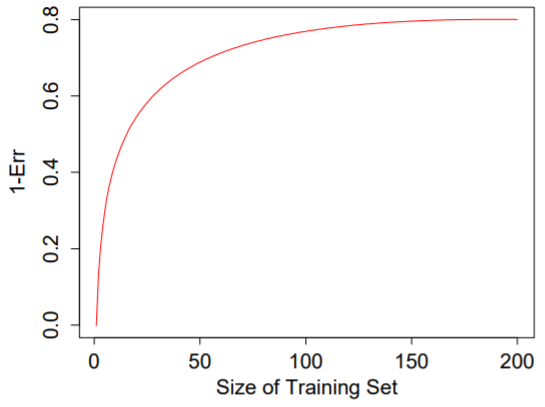
\includegraphics[width=0.4\textwidth]{chapters/regularization.model.selection/figures/learning_curve.png}
	\caption{\textbf{Learning Curve of classifier}: showing the success ($1-Err$) as a function of the training set size}
	\label{learning_curve}
\end{figure}
\subsubsection{Under-estimating Generalization Error}
A much more common mistake is being too optimistic in estimating the generalization error, causing under-estimation of it. Suppose we are given a learning problem and a dataset with $m$ samples. We begin trying different types of models, each with its own tuning parameters. Perhaps we also alter the training sample $S$ by removing- or adding features and addressing ``problematic`` samples. Eventually we have a ``clean`` training sample and a tuned model that works well. Now we perform model evaluation to estimate the generalization error of the chosen learner.
\\~\\
In such a scenario we will end up under-estimating the generalization error due to two mistakes:
\begin{itemize}
	\item The first is known as \textbf{model snooping}. By trying out many learners, tuning the parameters of each and looking for one model that will perform very well, we slowly begin overfitting to the training sample. Each time we discarded some potential hypothesis class in favor of another that performed better we introduced more bias to the procedure. Even in the case where we use a validation set, if we evaluate the performance over it many times, we begin overfitting to it as well.
	\item The second is known as \textbf{data snooping}. Once we evaluate our selected model over a new test sample ()or perhaps even when using it in production) this data did not under-go the same level of treatment. It might contain missing features or ``problematic`` samples that were dealt with in $S$. Therefore, the cross-validation procedure will under-estimate the generalization error over the new data.
\end{itemize}
~\\
To avoid this problem we should deal with these types of snooping. Limit model- and data- snooping to a small subset of $S$ which will be ``contaminated with optimism``. Use it to get general understanding of the data and potential models. Only once the snooping stage has completed and a small set of candidate learners is chosen, use the entire training set for model selection- and evaluation. In addition, avoid manual data snooping. \textbf{Code the entire pre-processing stage}. At each iteration of Bootstap of cross-validation run the eintire pre-processing step over the current sample, just like it would run when predicting over new data.

\section{Summary}
\subsection{Lab: Selecting Regularized Model}
\subsection{Lab: Regularized Logistic Regression}